\section{The Least Mean Square (LMS) Algorithm}

\begin{enumerate}[label=\alph*), leftmargin=*]

%% a)
\item
%

A general AR(2) process $x(n)$ with parameters $a_{1}, a_{2}$ satisfies the difference equation:

\begin{equation}
    x(n) = a_{1} x(n - 1) + a_{2} x(n - 2) + \eta(n)
\label{eq:ar_2}
\end{equation}

where $\eta(n) \sim \mathcal{N}(0, \sigma_{\eta}^{2})$. The Least Mean Square (LMS) algorithm is used to approximate
the autoregressive parameters $a_{1}, a_{2}$ from data, treating $\mathbf{x}(n) = [x(n-1), x(n-2)]^{T}$ and
$y(n) = x(n)$ as the input (features) vector and the output (target), respectively.

The correlation matrix $\mathbf{R}_{xx}$ of the input vector $\mathbf{x}(n)$ is given by:

\begin{equation}
    \mathbf{R}_{xx} = \E[\mathbf{x}(n) \mathbf{x}^{T}(n)] = \E
    \begin{bmatrix}
        x(n-1) x(n-1) & x(n-1) x(n-2) \\
        x(n-1) x(n-2) & x(n-2) x(n-2)
    \end{bmatrix} =
    \begin{bmatrix}
        r_{xx}(0) & r_{xx}(1) \\
        r_{xx}(1) & r_{xx}(0)
    \end{bmatrix}
\label{eq:cov_ar_2}
\end{equation}

where $r_{xx}(k)$ the autocorrelation function (ACF) of $x(n)$. To obtain the ACF of the AR(2) process, multiply equation (\ref{eq:ar_2}) by $x(n-k)$ and take expectations:

\begin{align}
    r_{xx}(k) = \E[ x(n) x(n-k) ]   &= \E \bigg[ a_{1} x(n - 1) x(n-k) + a_{2} x(n - 2) x(n-k) + \eta(n) x(n-k) \bigg] \nonumber\\
    r_{xx}(k) = \E[ x(n) x(n-k) ]   &= a_{1} \E \big[ x(n - 1) x(n-k) \big] + a_{2} \E \big[ x(n - 2) x(n-k) \big] + \E \big[ \eta(n) x(n-k) \big]
\end{align}

Notice that $\E [\eta(n) x(n-k)]$ vanishes when $k > 0$, then:

\begin{align}
    r_{xx}(0)   &= a_{1} r_{xx}(1) + a_{2} r_{xx}(2) + \sigma_{\eta}^{2} \\
    r_{xx}(k)   &= a_{1} r_{xx}(k-1) + a_{2} r_{xx}(k-2), k > 0
\label{eq:acf_ar_2}
\end{align}

Note that ACF is an even function or equivalently $r_{xx}(-k) = r_{xx}(k), \forall k \in \sZ$, thus using the true process parameters $a_{1} = 0.1$, $a_{2} = 0.8$
and $\sigma_{\eta}^{2} = 0.25$, we obtain the three simultaneous equations with three unknowns:

\begin{align}
    r_{xx}(0)   &= a_{1} r_{xx}(1) + a_{2} r_{xx}(2) + \sigma_{\eta}^{2} \\
    r_{xx}(1)   &= a_{1} r_{xx}(0) + a_{2} r_{xx}(-1) = a_{1} r_{xx}(0) + a_{2} r_{xx}(1) \\
    r_{xx}(2)   &= a_{1} r_{xx}(1) + a_{2} r_{xx}(0)
\end{align}

with the unique solution $r_{xx}(k) = [\frac{25}{27}, \frac{25}{54}, \frac{85}{108}]$ for $k=1, 2, 3$.

Hence by substitution in equation (\ref{eq:cov_ar_2}) we obtain the  correlation matrix of the input vector $\mathbf{x}(n)$:

\begin{equation}
    \mathbf{R}_{xx} = 
    \frac{25}{54}
    \begin{bmatrix}
        2 & 1 \\
        1 & 2
    \end{bmatrix}
\label{eq:cov_ar_2_result}
\end{equation}

Convergence of the LMS algorithm depends on the step size $\mu$, which should satisfy:

\begin{equation}
    0 < \mu < \frac{2}{\lambda_{max}}
\label{cond:mu_max}
\end{equation}

where $\lambda_{max}$ the largest eigenvalue of the correlation matrix $\mathbf{R}_{xx}$. Performing the eigendecomposition of $\mathbf{R}_{xx}$, we obtain
$\lambda_{1} = 0.4630$ and $\lambda_{2} = \lambda_{max} = 1.3889$ and as a result, convergence to the Wiener optimal solution is guaranteed for:

\begin{equation}
    0 < \mu < 1.44
\label{cond:mu_max_val}
\end{equation}

%% b)
\item
%

The LMS algorithm is implemented and tested on $N=1000$ samples of 100 different realisations of $x(n)$ process. The squared prediction error over time
for one and the average of the 100 realisations is provided at figure \ref{fig:3_1_b} for two different step-sizes $\mu_{1} = 0.01$ and $\mu_{2} = 0.05$.

\begin{figure}[h]
    \centering
    \begin{subfigure}{0.49\textwidth}
        \centering
        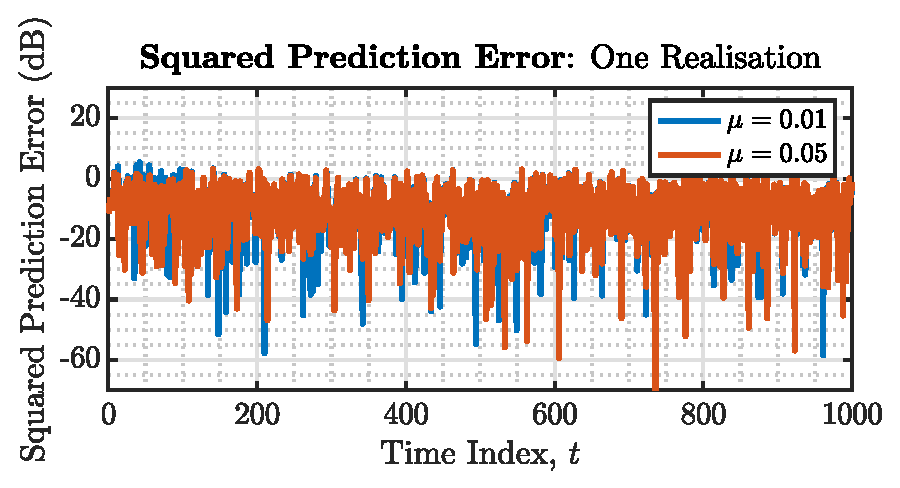
\includegraphics[height=1.5in]{report/adaptive-signal-processing/the-least-mean-square-algorithm/assets/b/squared_prediction_error_1}
    \end{subfigure}
    ~
    \begin{subfigure}{0.49\textwidth}
        \centering
        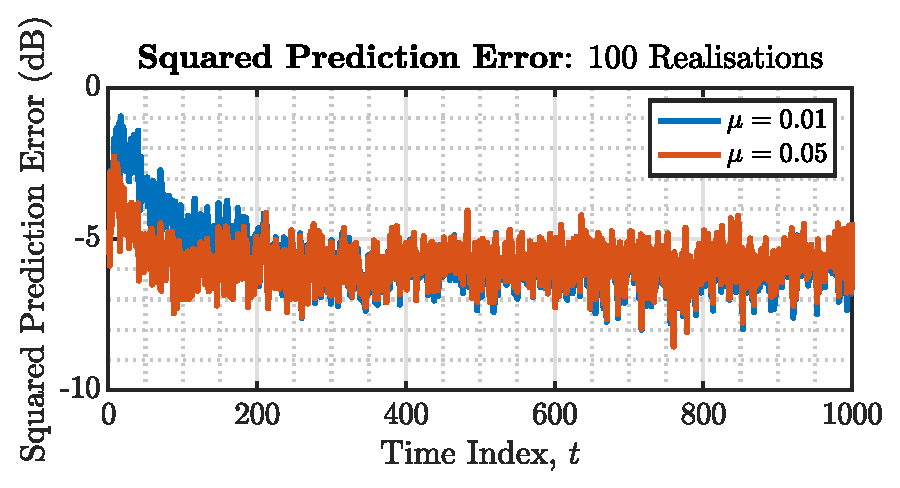
\includegraphics[height=1.5in]{report/adaptive-signal-processing/the-least-mean-square-algorithm/assets/b/squared_prediction_error_ens}
    \end{subfigure}
    \caption{LMS: squared prediction error over time and $\mu$ convergence rate.}
    \label{fig:3_1_b}
\end{figure}

Concentrating on the averaged of 100 realisation prediction error (reduced variance of estimate), we notice that the larger step-size $\mu_{2} = 0.05$ converges
within 50 timesteps, while $\mu_{1}$ converges in 200 timesteps, verifying the theoretical argument that larger $\mu$ values allow steeper decent of the error surface,
as long as the condition (\ref{cond:mu_max_val}) is satisfied. Nonetheless, fast convergence is traded with larger oscillations around the true parameter values,
motivating the use of an adaptive step-size, which decays over time.

%% c)
\item
%

The theoretical Misadjustment, $\mathcal{M}_{LMS}$, of the LMS algorithm is obtained by the approximation formula:

\begin{equation}
    \mathcal{M}_{LMS} \approx \frac{\mu}{2} Tr\{ \mathbf{R}_{xx} \} = \frac{\mu}{2} 1.8519
\end{equation}

where $\mathbf{R}_{xx}$ from (\ref{eq:cov_ar_2_result}) is used.

According to figure \ref{fig:3_1_b} the squared prediction error plateaus for both $\mu$ values after $t > 200$. To guarantee that a steady-state has been reached,
we time average the squared prediction error for $t_{0} > 500$, in order to obtain a Mean Squared Error (MSE) estimate. The empirical misadjustment, $\mathcal{M}_{emp}$,
is then obtained using the formula:

\begin{equation}
    \mathcal{M}_{emp} = \frac{\mathtt{MSE}}{\sigma_{\eta}^{2}} - 1
\end{equation}

Table \ref{tab:3_1_c} summarises the empirical and theoretical misadjustments of the simple LMS algorithm for the $x(n)$ process.

\begin{table}[h]
\centering
\begin{tabular}{|c|c|c|}
\hline
$\boldsymbol{\mu}$ & $\mathcal{M}_{LMS}$ & $\mathcal{M}_{emp}$ \\
\hline
\hline
$0.01$ & $0.0093$ & $0.00766$ \\
\hline
$0.05$ & $0.0463$ & $0.04912$ \\
\hline
\end{tabular}
\caption{LMS: empirical and theoretical approximation of misadjustment comparison matrix.}
\label{tab:3_1_c}
\end{table}

%% d)
\item
%

The evolution of the LMS filter coefficients over time is shown in figure \ref{fig:3_1_d}, along with the true AR(2) process parameters, for step-sizes $\mu_{1} = 0.01$ and $\mu_{2} = 0.05$.
The illustrated curves represent the average of the coefficients of 100 independently trained LMS filters on different realisations of the same $x(n)$ stochastic process.

Clearly, for both $\mu$ values, $\hat{a}_{1}$ coefficient converges to the true $a_{1}$ parameter, while the second coefficient $\hat{a}_{2}$ has a negative offset
($3.75\%$ for $\mu_{1} = 0.01$ and $10\%$ for $\mu_{2} = 0.05$). Moreover, we note that a larger step-size (i.e $\mu_{2}$) compromises oscillations around the true values and a greater offset
for faster convergence. In more detail, within 200 timesteps $\mu_{1}$ reaches the $10\%$ error bounds, while $\mu_{2}$ needs 350 timesteps.

\begin{figure}[h]
    \centering
    \begin{subfigure}{0.49\textwidth}
        \centering
        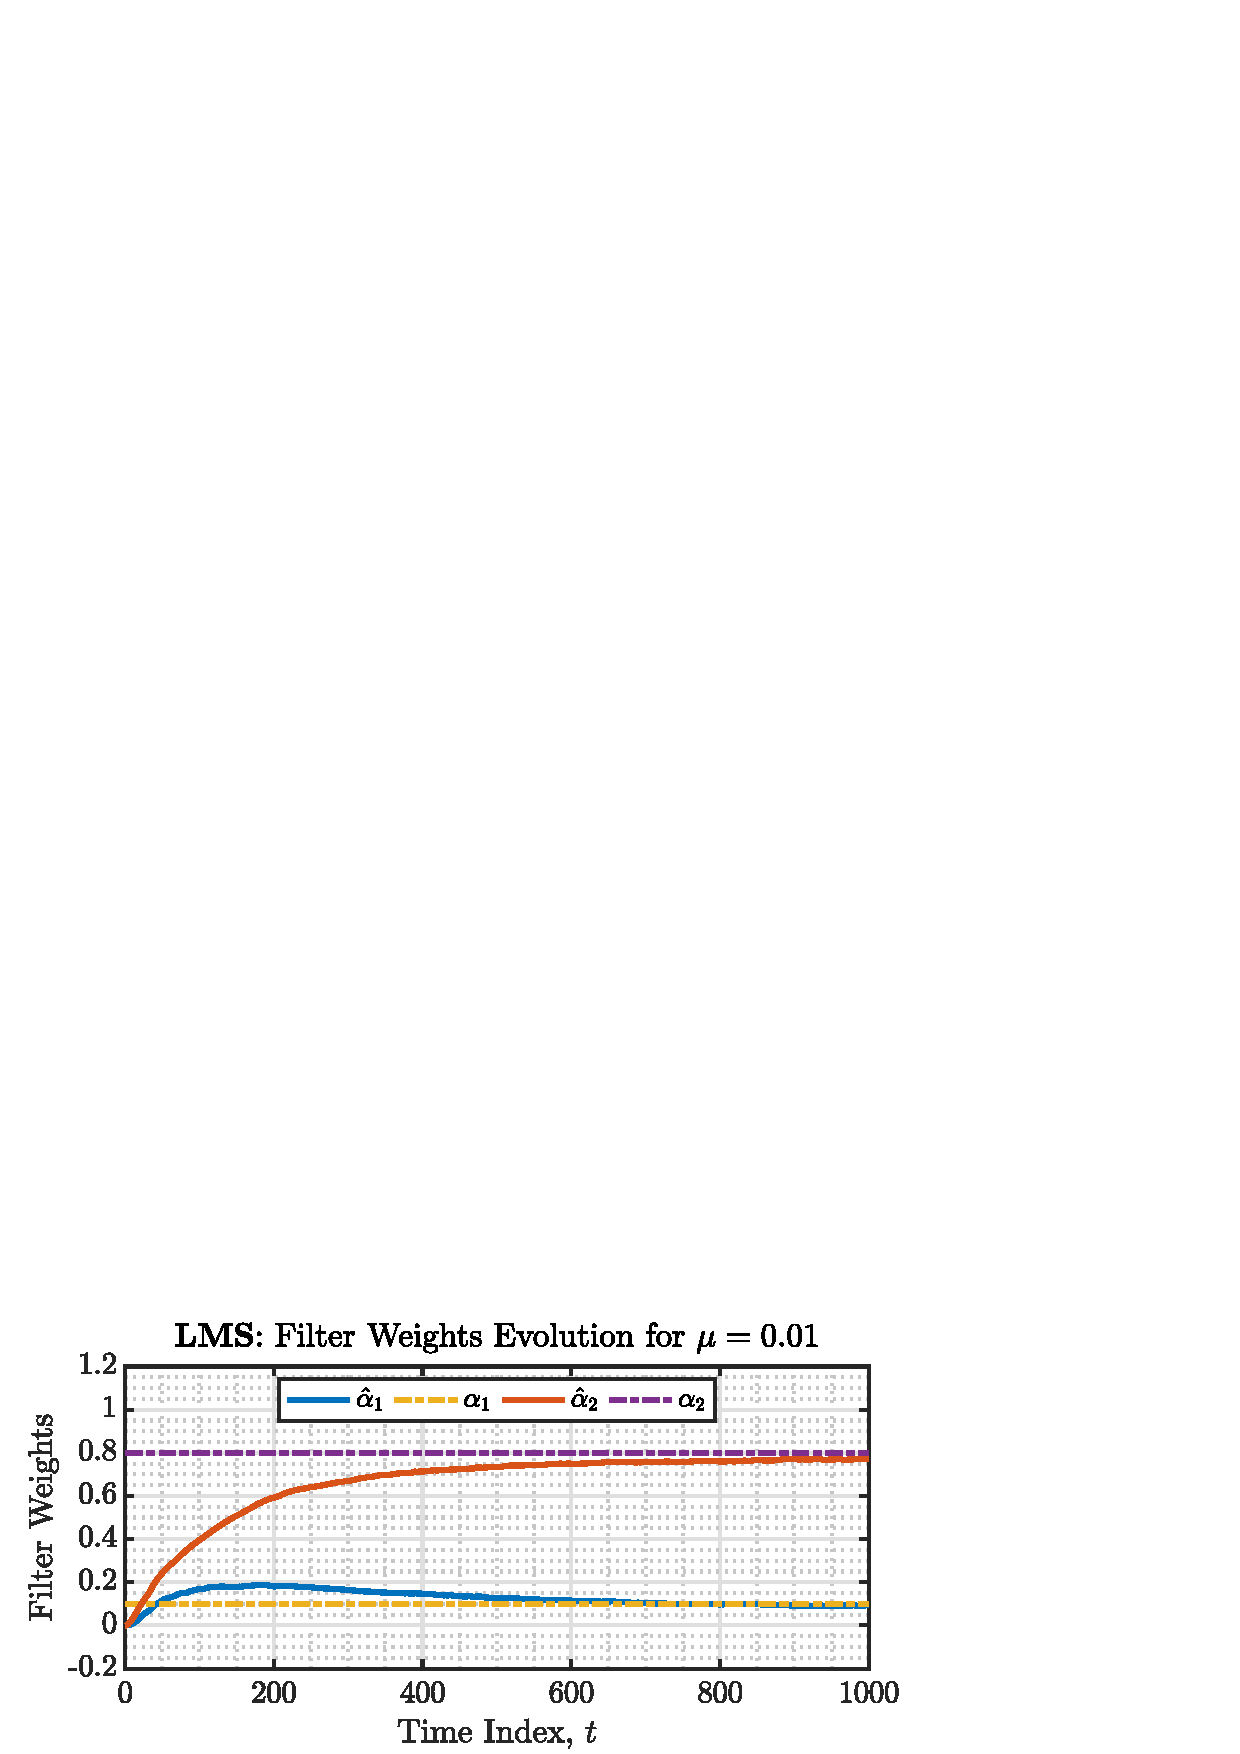
\includegraphics[height=1.5in]{{report/adaptive-signal-processing/the-least-mean-square-algorithm/assets/d/weights_evolution-mu_0.01}.pdf}
    \end{subfigure}
    ~
    \begin{subfigure}{0.49\textwidth}
        \centering
        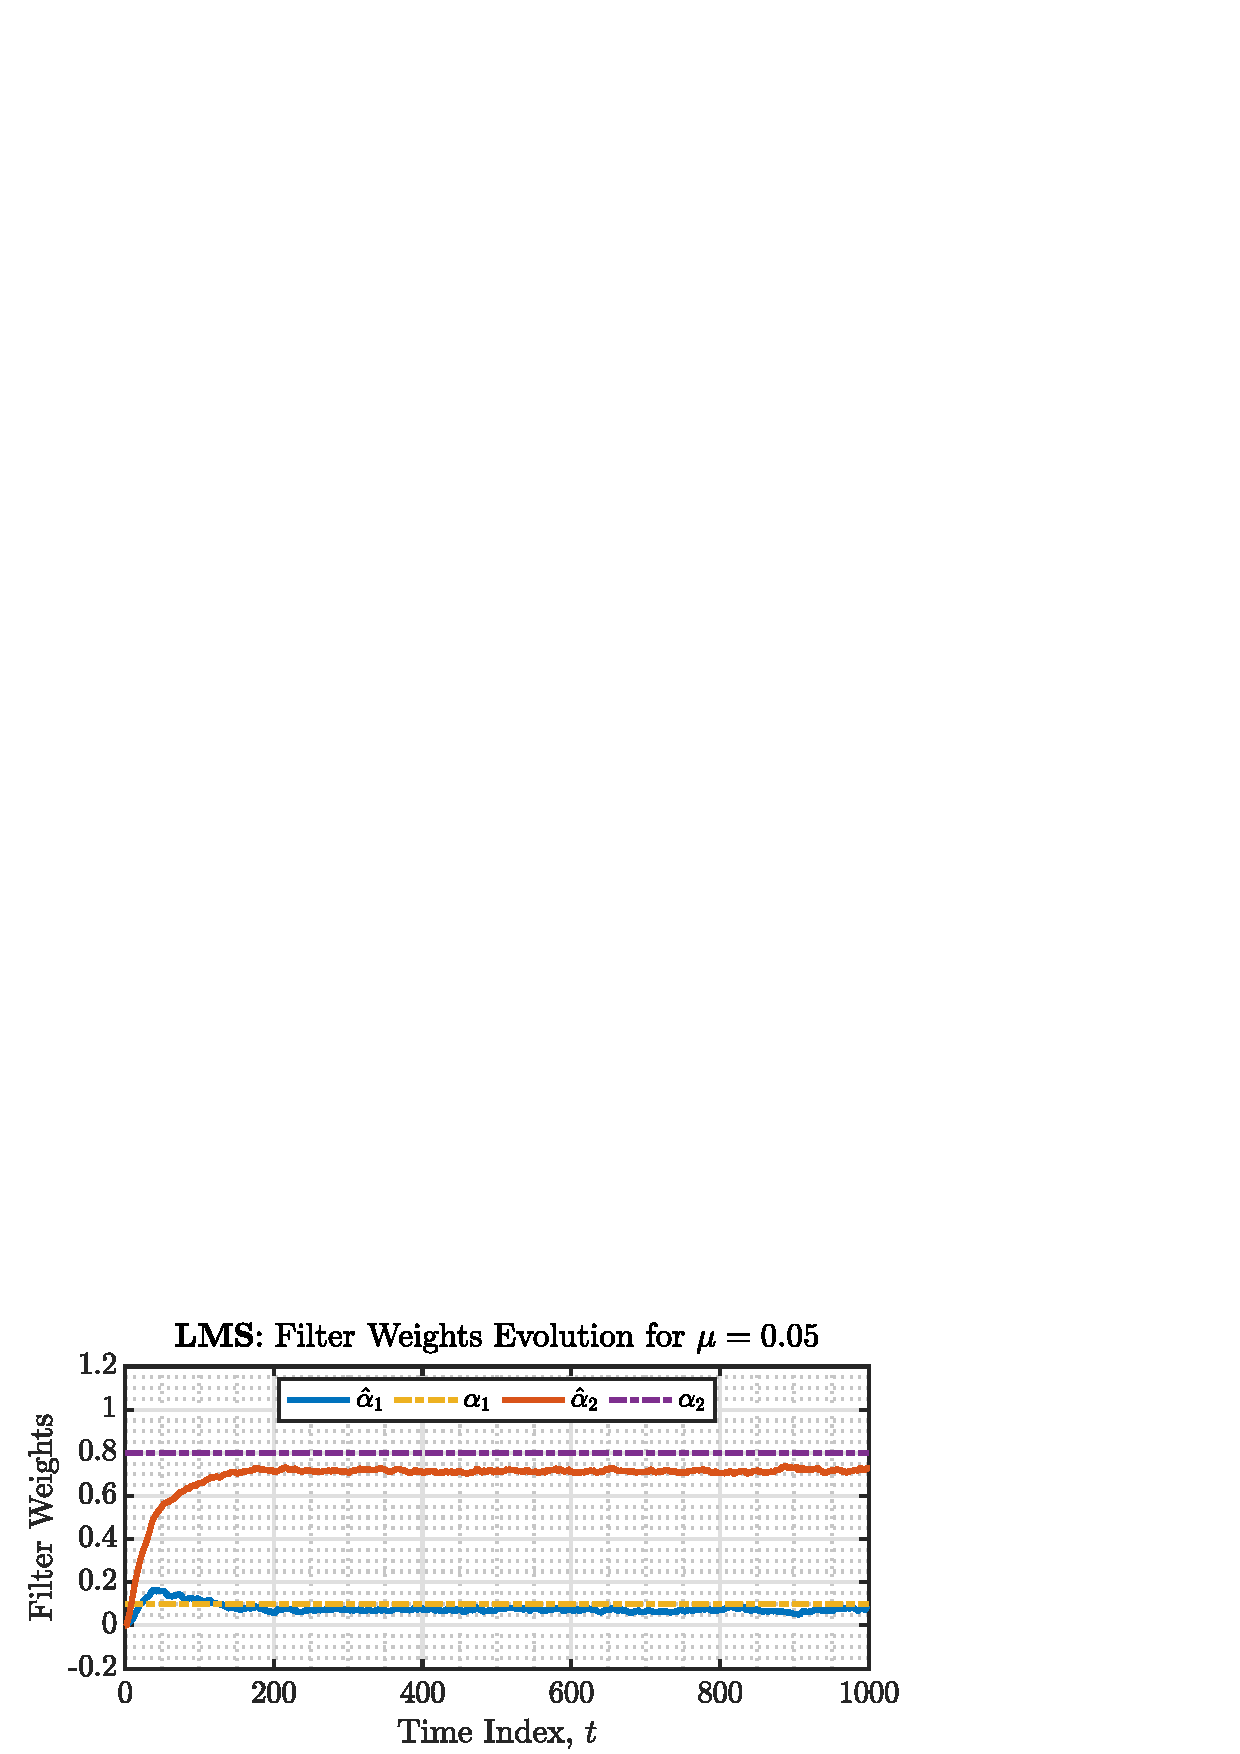
\includegraphics[height=1.5in]{{report/adaptive-signal-processing/the-least-mean-square-algorithm/assets/d/weights_evolution-mu_0.05}.pdf}
    \end{subfigure}
    \caption{LMS: steady state values of the adaptive filter coefficients for different step-sizes $\mu$.}
    \label{fig:3_1_d}
\end{figure}

%% e)
\item
%

Let the objective function $\mathcal{J}_{2}$, such that:

\begin{equation}
    \mathcal{J}_{2}(n) = \frac{1}{2} \bigg( e^{2}(n) + \gamma \| \vw(n) \|_{2}^{2} \bigg)
\label{eq:J_2}
\end{equation}

Expressing the error term, $e(n)$, in terms of the input vector $\mathbf{x}_{n}$ and the target value $y_{n}$:

\begin{align}
    \mathcal{J}_{2}(n)  &= \frac{1}{2} \bigg( \| y(n) - \vw(n)^{T} \mathbf{x}(n) \|_{2}^{2} + \gamma \| \vw(n) \|_{2}^{2} \bigg) \\
    \mathcal{J}_{2}(n)  &= \frac{1}{2} \bigg( \big( y(n) - \vw(n)^{T} \mathbf{x}(n))^{T} (y(n) - \vw(n)^{T} \mathbf{x}(n) \big) + \gamma \vw(n)^{T} \vw(n) \bigg)
\end{align}

Calculating the gradient of the objective function, $\nabla_{\vw} \mathcal{J}_{2}$, with respect to the weights $\vw$:

\begin{align}
    \nabla_{\vw} \mathcal{J}_{2}(n) &= - ( y(n) - \vw(n)^{T} \mathbf{x}(n) ) \mathbf{x}(n) + \gamma \vw(n) \\
    \nabla_{\vw} \mathcal{J}_{2}(n) &= - e(n) \mathbf{x}(n) + \gamma \vw(n)
\end{align}

Applying the gradient descent update to weights $\vw$ to minimise the objective function $\mathcal{J}_{2}$:

\begin{align}
    \vw(n + 1)  &= \vw(n) - \mu \nabla_{\vw} \mathcal{J}_{2}(n) \\
    \vw(n + 1)  &= \vw(n) - \mu \big( - e(n) \mathbf{x}(n) + \gamma \vw(n) \big) \\
    \vw(n + 1)  &= (1 - \mu \gamma) \vw(n) + \mu e(n) \mathbf{x}(n)
\label{eq:leaky_lms}
\end{align}

Hence we proved that the Leaky LMS algorithm following the update rule in (\ref{eq:leaky_lms}) is equivalent to the minimisation of the objective function $\mathcal{J}_{2}$
defined in (\ref{eq:J_2}).

%% f)
\item
%

In figure \ref{fig:3_1_f} the Leaky LMS filter coefficients for different leakage coefficient $\gamma$ and step-sizes $\mu$
are provided, against the true AR(2) process parameters.

The predicted filter coefficients do not converge to the true parameters, and increasing $\gamma$ values introduce
a greater bias between the estimates and the process autoregressive parameters.

The offline, non-adaptive but optimal solution to this linear system is the Wiener filter, which has access to all the
observed samples and relies on the construction of the autocorrelation matrix, $\mathbf{R} = \E [ \mathbf{X} \mathbf{X}^{T} ]$,
and the crosscorrelation vector (between desired output value and input vector), $\mathbf{p}$, then the optimal filter weights,
$\vw_{*}$, are given by:

\begin{equation}
    \vw_{*} = \mathbf{R}^{-1} \vp
\end{equation}

where $\mathbf{R}$ needs to be invertible. The LMS algorithm can be shown to converge to this solution if (\ref{cond:mu_max})
is true. Invertibility of the autocorrelation matrix is not guaranteed, since it is positive semi-definite and not strictly
positive definite. The Leaky LMS algorithm can be shown to converge to the solution:

\begin{equation}
    \vw_{reg} = (\mathbf{R} + \gamma \mathbf{I})^{-1} \vp
\end{equation}

where the leakage coefficient $\gamma > 0$ acts as a regularization parameter ensuring invertibility of the "modified"
autocorrelation matrix $(\mathbf{R} + \gamma \mathbf{I})$. Nonetheless, this is a common example of bias-variance trade-off
since larger values of $\gamma$ introduce bias but penalise variance of estimates
(due to the $L_{2}$ norm term in $\mathcal{J}_{2}$).

\begin{figure}[h]
    \centering
    \begin{subfigure}{0.49\textwidth}
        \centering
        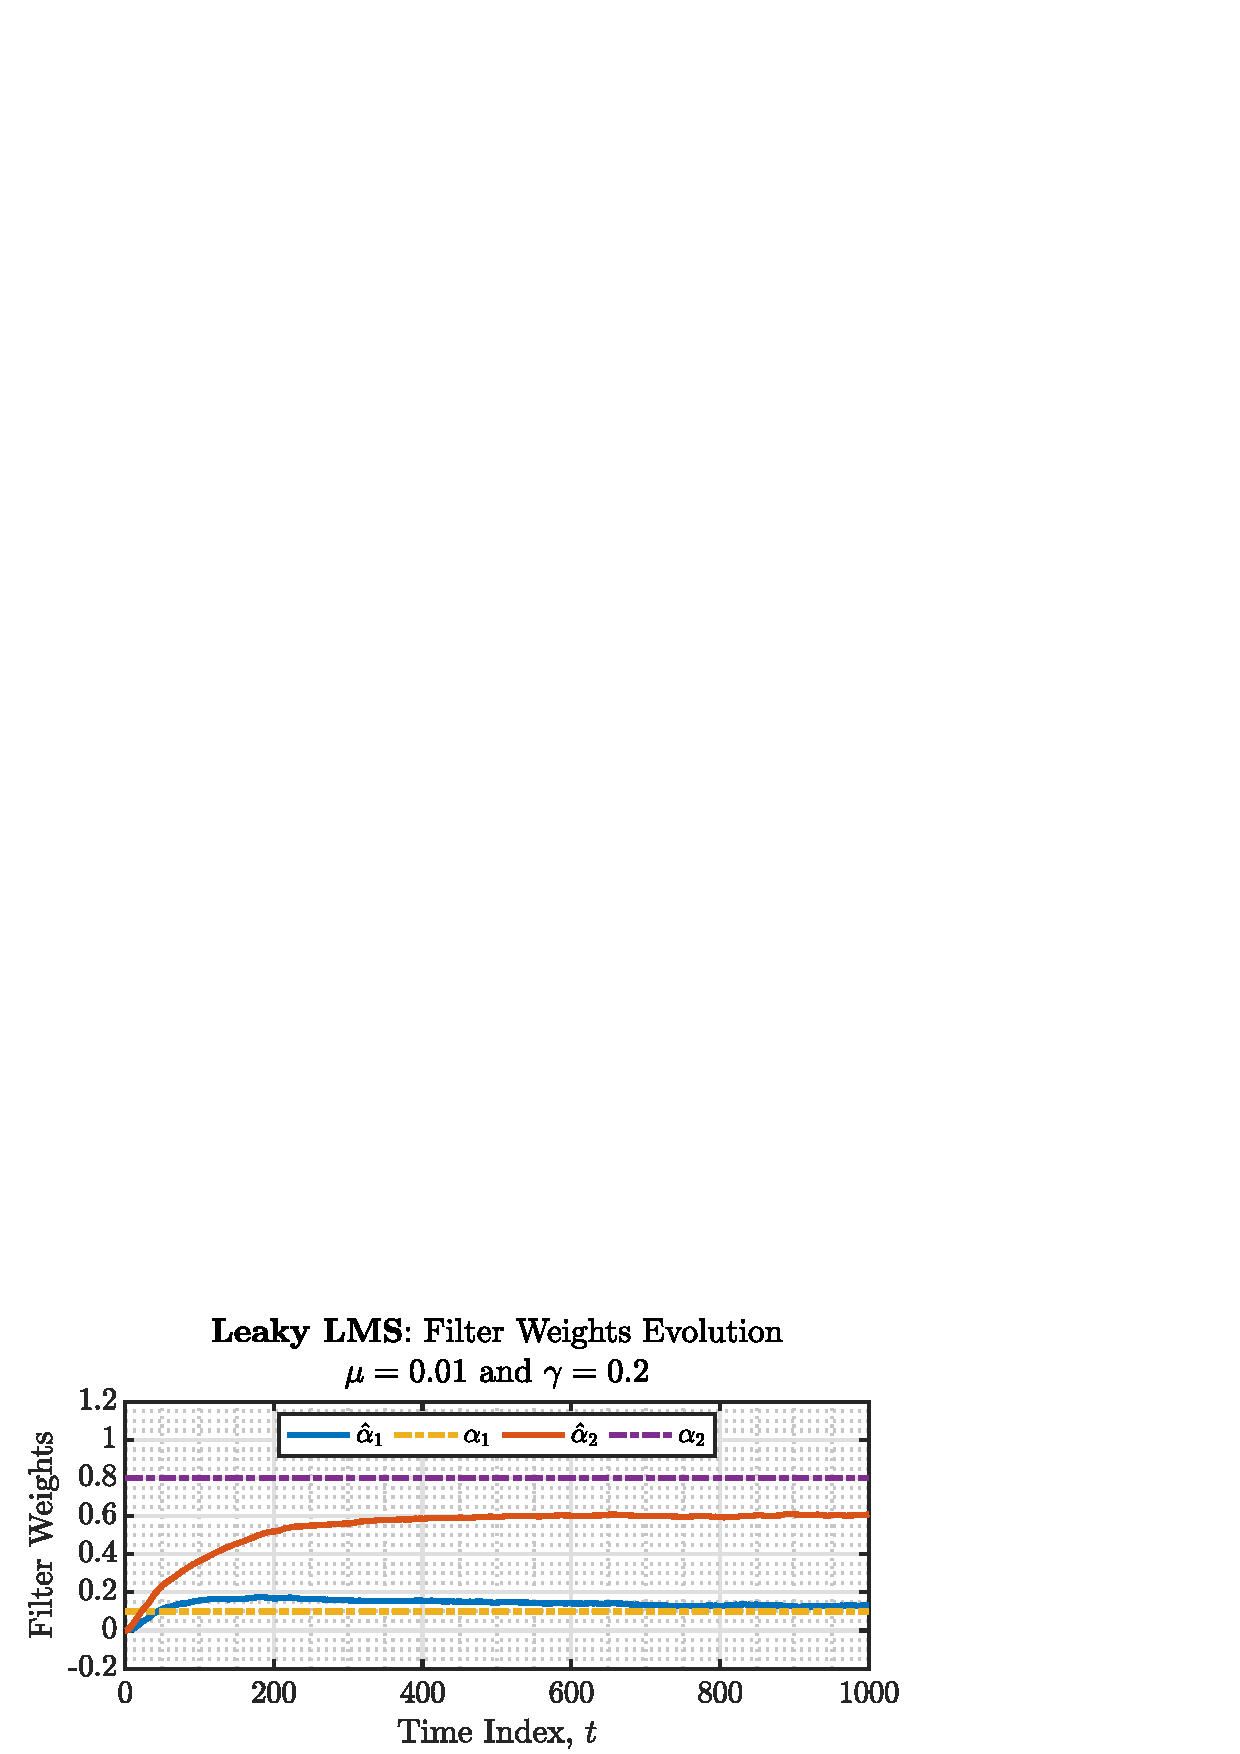
\includegraphics[height=1.5in]{{report/adaptive-signal-processing/the-least-mean-square-algorithm/assets/f/weights_evolution-mu_0.01-gamma_0.2}.pdf}
    \end{subfigure}
    ~
    \begin{subfigure}{0.49\textwidth}
        \centering
        \includegraphics[height=1.5in]{{report/adaptive-signal-processing/the-least-mean-square-algorithm/assets/f/weights_evolution-mu_0.05-gamma_0.2}.pdf}
    \end{subfigure}
    ~
    ~
    \begin{subfigure}{0.49\textwidth}
        \centering
        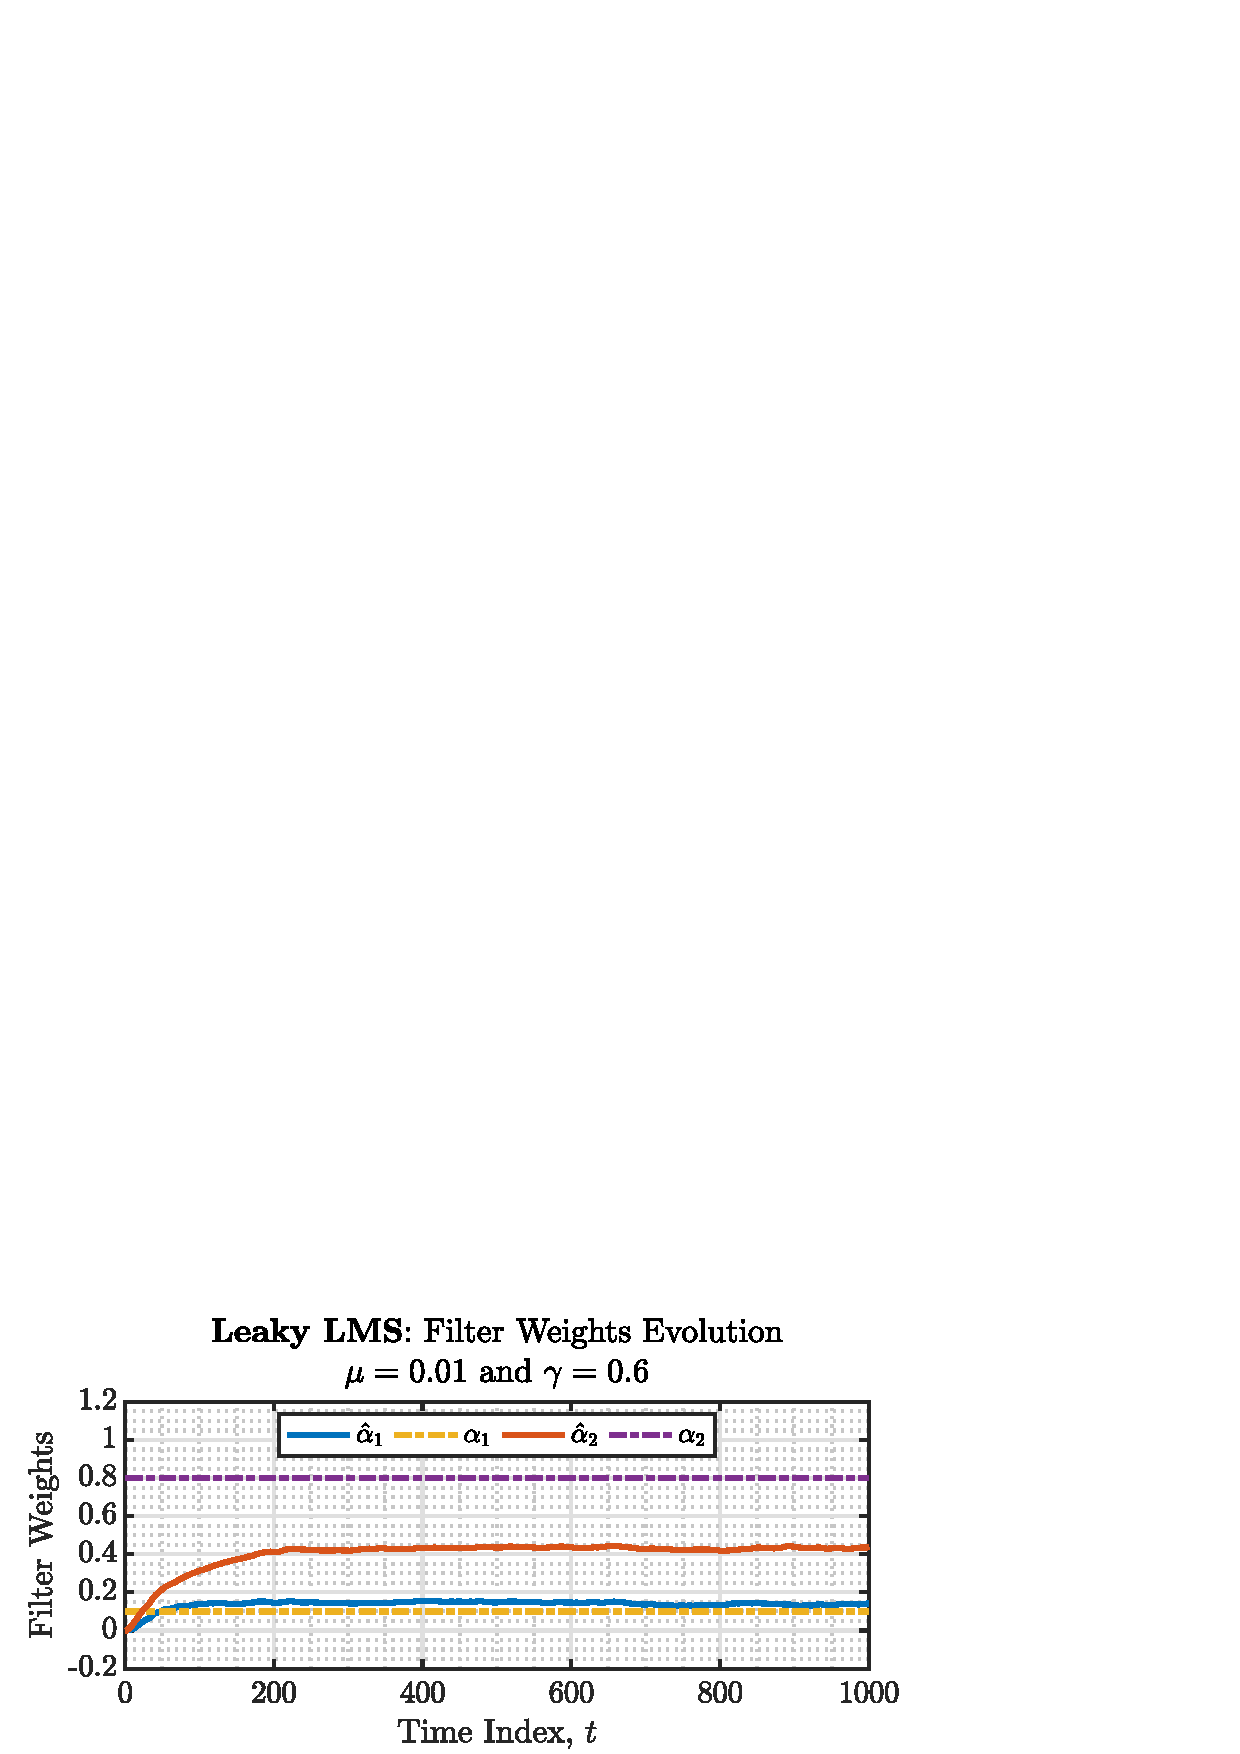
\includegraphics[height=1.5in]{{report/adaptive-signal-processing/the-least-mean-square-algorithm/assets/f/weights_evolution-mu_0.01-gamma_0.6}.pdf}
    \end{subfigure}
    ~
    \begin{subfigure}{0.49\textwidth}
        \centering
        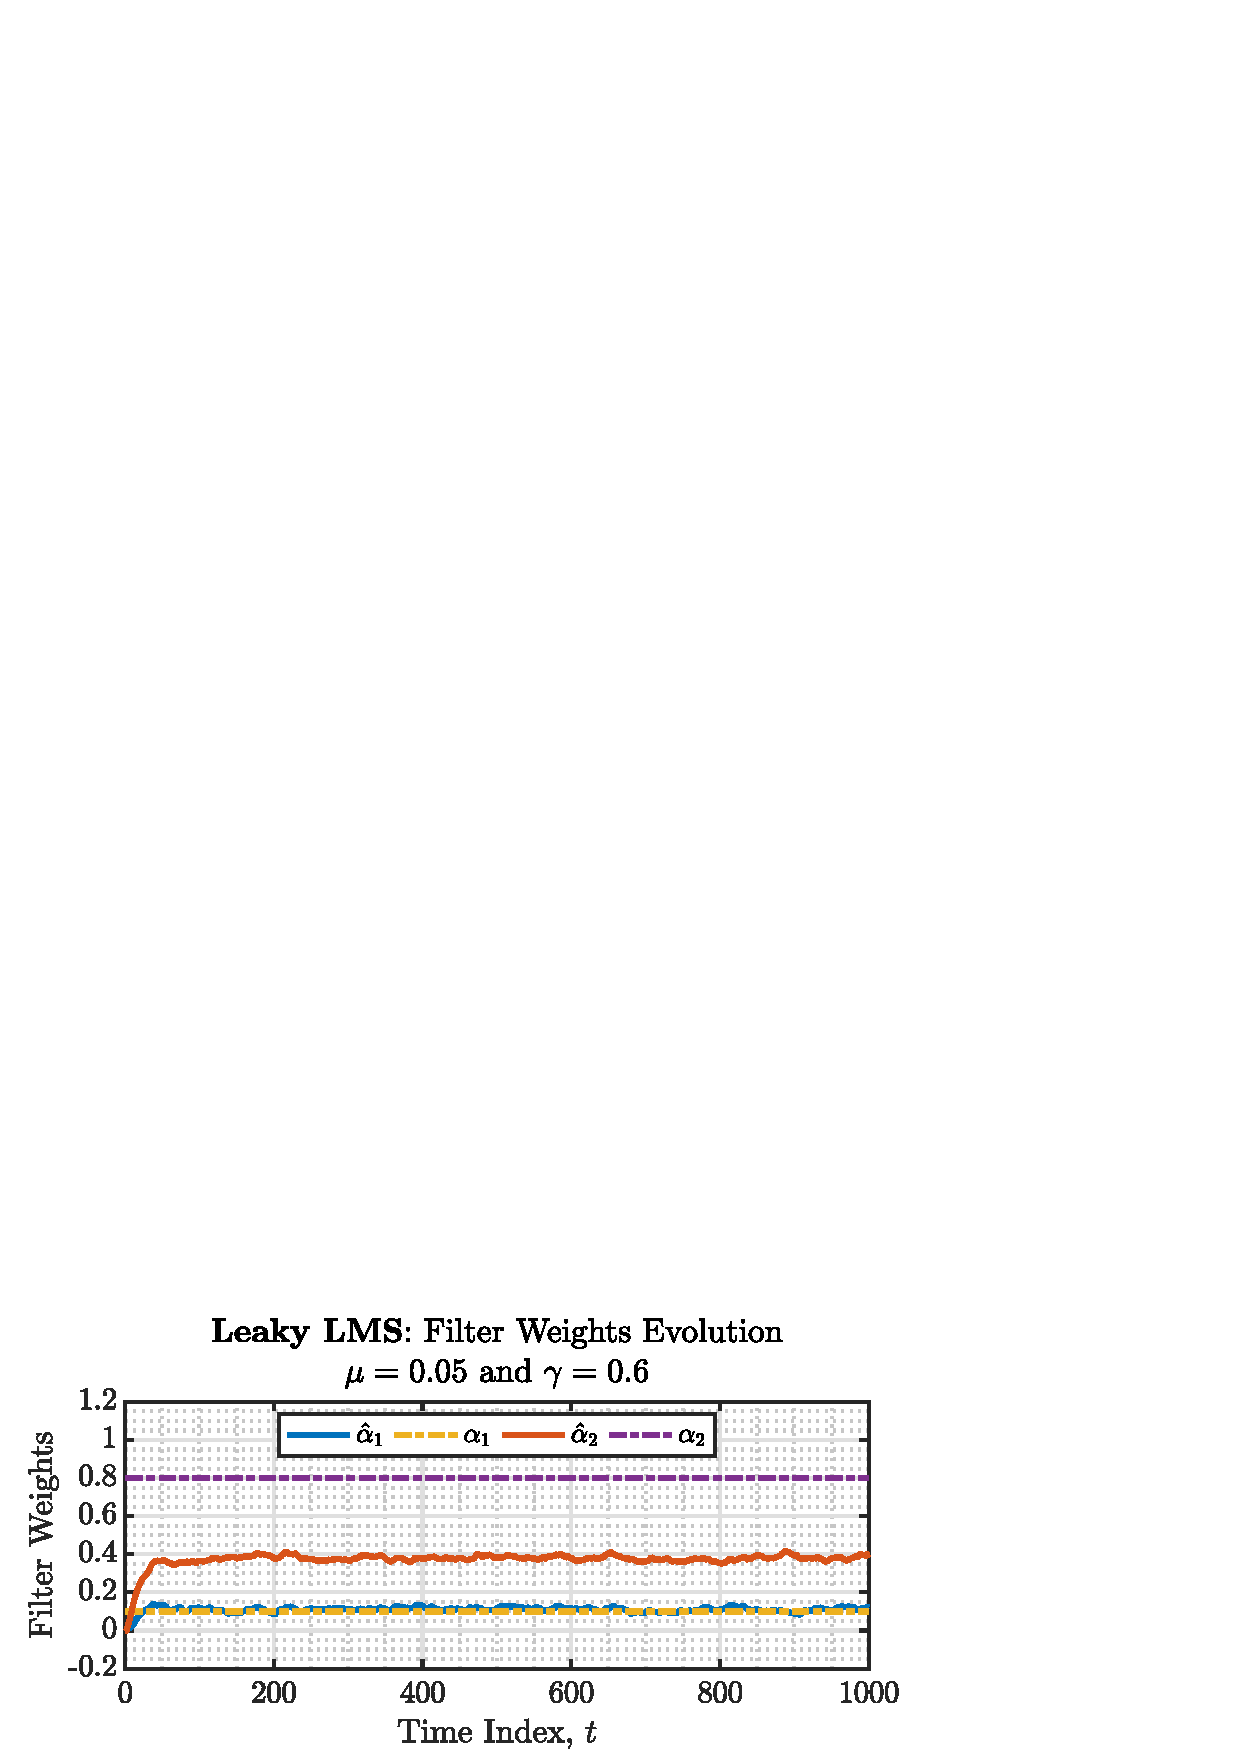
\includegraphics[height=1.5in]{{report/adaptive-signal-processing/the-least-mean-square-algorithm/assets/f/weights_evolution-mu_0.05-gamma_0.6}.pdf}
    \end{subfigure}
    ~
    ~
    \begin{subfigure}{0.49\textwidth}
        \centering
        \includegraphics[height=1.5in]{{report/adaptive-signal-processing/the-least-mean-square-algorithm/assets/f/weights_evolution-mu_0.01-gamma_1.0}.pdf}
    \end{subfigure}
    ~
    \begin{subfigure}{0.49\textwidth}
        \centering
        \includegraphics[height=1.5in]{{report/adaptive-signal-processing/the-least-mean-square-algorithm/assets/f/weights_evolution-mu_0.05-gamma_1.0}.pdf}
    \end{subfigure}
    \caption{Leaky LMS: filter weights evolution for different leakage coefficient $\gamma$.}
    \label{fig:3_1_f}
\end{figure}

%
\end{enumerate}